\chapter{济南市丁家庄城中村照片集}

\thispagestyle{empty}本章图片均为笔者拍摄于丁家庄城中村,采用了如实摄影(straight photography)的拍摄手法,力图直接呈现丁家庄的生态,让其为自己发声。

\vspace{2cm}
\begin{figure}[!ht]
  \centering
  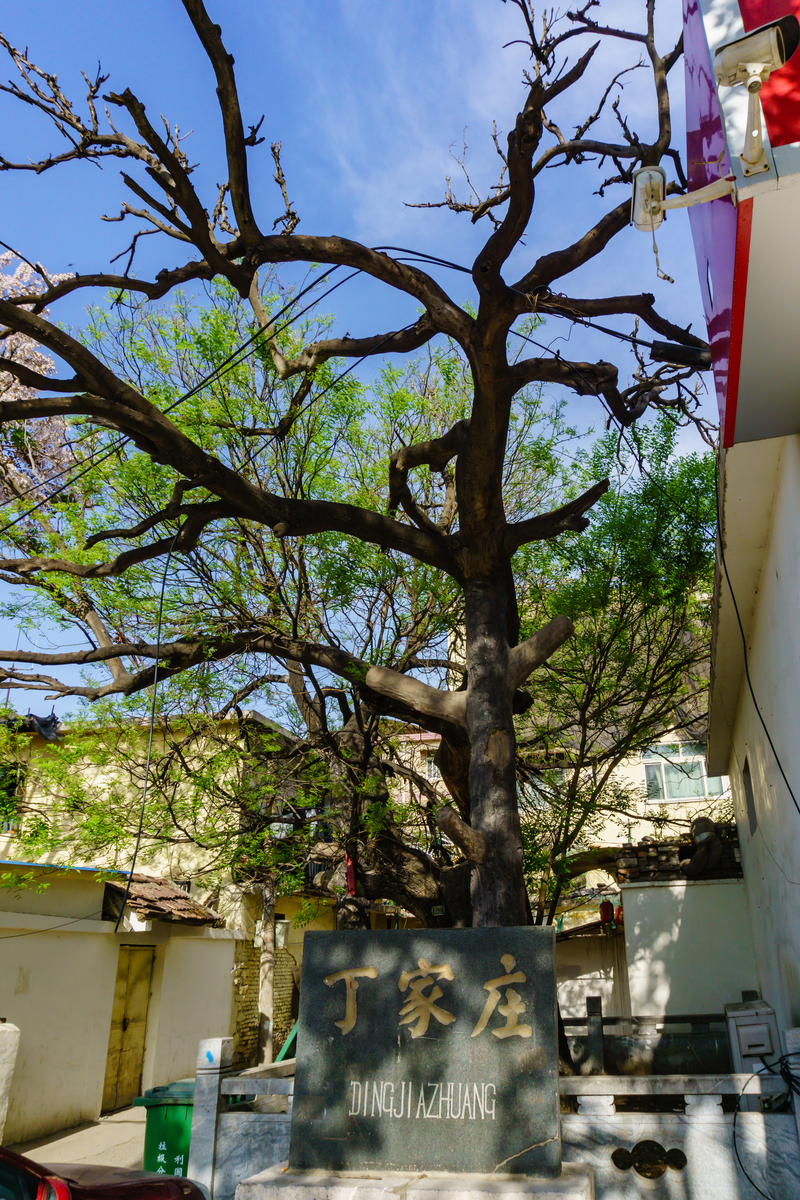
\includegraphics[keepaspectratio, height = 0.6\textheight]{dingjia/cunbei.jpg}
  \caption{丁家庄村碑}
  \label{fig:cunbei} % \raggedright \raggedright \small 2017年4月20日,丁家庄村口的村碑和百年老槐树。
\end{figure}
\clearpage


\dingphotoh{sanbadaji}{熙熙攘攘的三八大集}{2017年5月8日,丁家庄每逢农历三、八为大集。}{zuwu1}{北侧一处出租楼房外景}{2017年4月7日}

\dingphotov{guodao1}{一条街道}{2017年4月7日。}

\dingphotoh{guzhai}{城中村最为破败的一间自搭棚户}{2017年5月6日}{bizhezuwu}{笔
  者田野调查中租住的单间}{2017年4月25日,月租金240元,网络费30元,居住条件在
  城中村属于中等偏上。}

\dingphotov{chucangshi}{夫妻二人和他们一岁孩子所租住的储藏室}{2017年4月15日}

\dingphotov{cesuo1}{城中村中等水平的简易卫生间}{2017年3月31日,这类卫生间多为
  房东所建,常常加锁,只供其名下租客使用。}

\dingphotoh{yangguang}{阳光}{2017年4月26日,木制挂锁卫生间。}{lou1}{二楼房顶
  私搭简易板房}{2016年11月20日}

\dingphotov{shaoshui}{丁家庄村民常用的木柴铁皮桶炉}{2017年5月8日,丁家庄一些
  村民为节俭持家常用这种简易炉烧开水,火力弱,耗时长、烟雾较大。}

\dingphotoh{youeryuan}{幼儿园外墙与线缆}{2017年3月31日。}{wanshua}{玩耍的孩子
  们}{拍摄于2017年5月7日。}

\dingphotov{jiagai}{改造楼梯、层层加盖的一座楼房}{拍摄于2017年5月11日}

\dingphotoh{jiejing2}{街景}{2017年3月26日}{caishichang}{丁家庄综合市场中的一
  处菜摊}{2017年4月26日,年租金近9万,年耗塑料袋1万元左右。虽然是大棚内的开放
  式摊位,租金比综合市场中的活动板房小吃店还要高不少。}

\dingphotoh{caitandajie1}{城中村内一处简易搭建的菜摊}{2016年12月14日,城中村
  内一处菜摊,这里并无租金。内有被褥,卖菜大姐应当也睡在这里。}
{caitandajie2}{简易菜摊消失了}{2017年3月8日,许是抵不住严寒和微薄收入,卖菜大
  姐和她的摊位不见了,只有床垫。}

\dingphotoh{zhian}{墙上张贴的治安告示}{2017年3月31日。这里盗窃案件可能略高于
  济南市其他小区,但远未达到恶劣的程度。笔者数十次进出丁家庄,未曾见过街头吵
  架斗殴。}{diushi}{一位走丢的小孩暂在三轮车摊主的怀抱中睡着}{拍摄
  于2016年11月09日,小孩从综合市场误入城中村,寻不见家长大哭不止,后在三轮车
  饮食摊主怀中睡着,身上披着他人提供的大衣。}

\dingphotoh{hua1}{一处住户外侧的绿植与杂物}{2017年4月12日。}{yangtai}{一处阳台——花与衣}{2017年4月12日。}

\dingphotov{cbd}{丁家庄工业南路南区一户未拆住房的外墙}{2017年4月20日,丁家庄南区是第一批拆除的宅基地住房,当时已达成动迁20余户,只余3户尚未动迁。}
